% !Mode:: "TeX:UTF-8" 

\BiSection{2.16}{Figures}

\fancyhead[R]{本题2.16由QC.Z完成}

考虑如图所示的结构,求$I_D$关于$V_{GS}$和$V_{DS}$的函数关系,并证明这一结构可看作宽长比等于$\frac{W}{2L}$的晶体管。假设$ \lambda = \gamma =0$。

		\begin{figure}[H] %H为当前位置,!htb为忽略美学标准,htbp为浮动图形
	\begin{minipage}{\linewidth}
		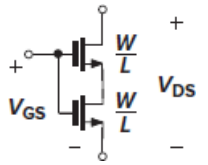
\includegraphics{2.16-t}
	\end{minipage}
\end{figure}

~~~~~~图2.55

解:

电路重画于图1

		\begin{figure}[H] %H为当前位置,!htb为忽略美学标准,htbp为浮动图形
	\begin{minipage}{\linewidth}
		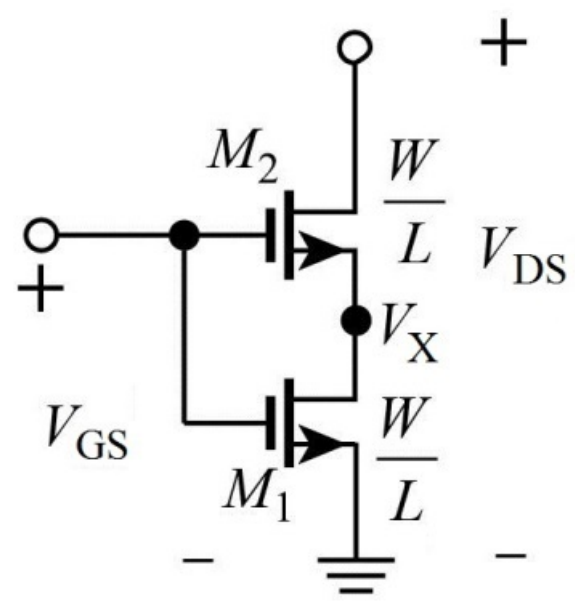
\includegraphics[width=1\linewidth]{2.16-1}
	\end{minipage}
	\caption*{图1} %最终文档中希望显示的图片标题
\end{figure}

\scalebox{3}{(1)}

NFET器件$M_1$在线性区。$V_{OD1}=V_{GS}-V_{TH},V_{DS1}=V_{X}$

NFET器件$M_2$在线性区。$V_{OD2}=V_{GS}-V_{X}-V_{TH},V_{DS2}=V_{DS}-V_{X}$

\begin{figure}[H] %H为当前位置,!htb为忽略美学标准,htbp为浮动图形
	\begin{minipage}{\linewidth}
		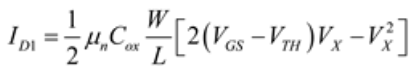
\includegraphics{2.16-2}
	\end{minipage}\ding{172}
\end{figure}

\begin{figure}[H] %H为当前位置,!htb为忽略美学标准,htbp为浮动图形
	\begin{minipage}{\linewidth}
		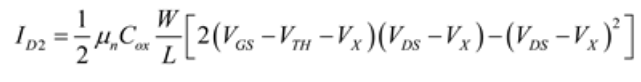
\includegraphics{2.16-3}
	\end{minipage}
\end{figure}

联立以上二式

\begin{figure}[H] %H为当前位置,!htb为忽略美学标准,htbp为浮动图形
	\begin{minipage}{\linewidth}
		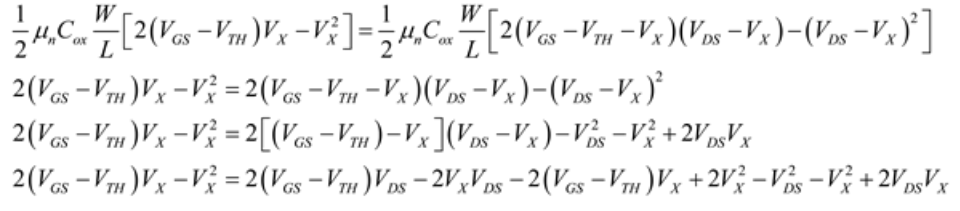
\includegraphics[width=1\linewidth]{2.16-4}
	\end{minipage}
\end{figure}

\begin{figure}[H] %H为当前位置,!htb为忽略美学标准,htbp为浮动图形
	\begin{minipage}{\linewidth}
		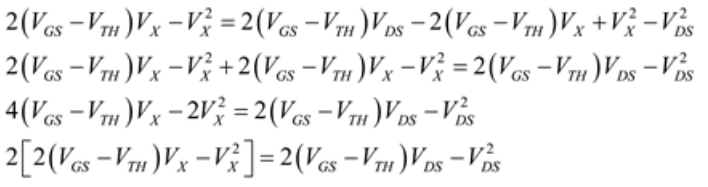
\includegraphics[width=1\linewidth]{2.16-5}
	\end{minipage}
\end{figure}

\begin{figure}[H] %H为当前位置,!htb为忽略美学标准,htbp为浮动图形
	\begin{minipage}{\linewidth}
		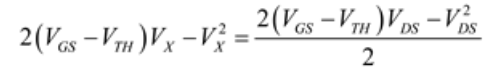
\includegraphics{2.16-6}
	\end{minipage}
\end{figure}

将上式代入\ding{172}

\begin{figure}[H] %H为当前位置,!htb为忽略美学标准,htbp为浮动图形
	\begin{minipage}{\linewidth}
		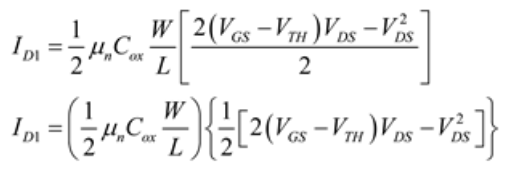
\includegraphics{2.16-7}
	\end{minipage}
\end{figure}

\begin{figure}[H] %H为当前位置,!htb为忽略美学标准,htbp为浮动图形
	\begin{minipage}{\linewidth}
		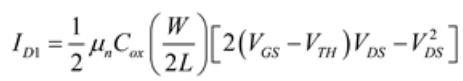
\includegraphics{2.16-8}
	\end{minipage}
\end{figure}

因为$I_{D1}=I_{D2}$,所以

\begin{figure}[H] %H为当前位置,!htb为忽略美学标准,htbp为浮动图形
	\begin{minipage}{\linewidth}
		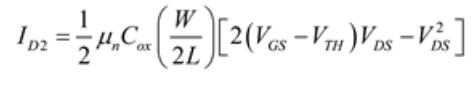
\includegraphics{2.16-9}
	\end{minipage}
\end{figure}

考虑原始线性区漏电流公式

\begin{figure}[H] %H为当前位置,!htb为忽略美学标准,htbp为浮动图形
	\begin{minipage}{\linewidth}
		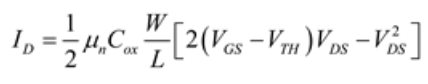
\includegraphics{2.16-10}
	\end{minipage}
\end{figure}

对比以上三式可得把整个图1电路视作一个晶体管时宽长比为$\frac{W}{2L}$。

\scalebox{3}{(2)}

$M_1$在线性区,$M_2$在饱和区。

\begin{figure}[H] %H为当前位置,!htb为忽略美学标准,htbp为浮动图形
	\begin{minipage}{\linewidth}
		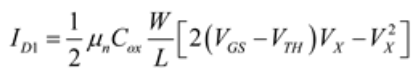
\includegraphics{2.16-11}
	\end{minipage}\ding{173}
\end{figure}

\begin{figure}[H] %H为当前位置,!htb为忽略美学标准,htbp为浮动图形
	\begin{minipage}{\linewidth}
		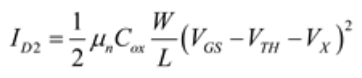
\includegraphics{2.16-12}
	\end{minipage}
\end{figure}

联立以上二式

\begin{figure}[H] %H为当前位置,!htb为忽略美学标准,htbp为浮动图形
	\begin{minipage}{\linewidth}
		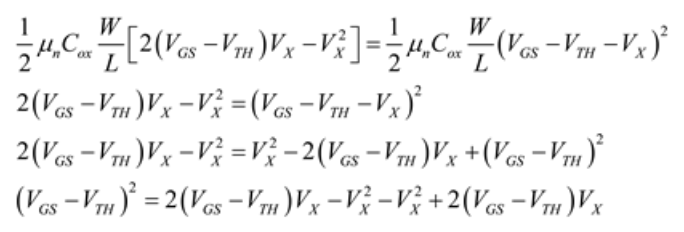
\includegraphics{2.16-13}
	\end{minipage}
\end{figure}

\begin{figure}[H] %H为当前位置,!htb为忽略美学标准,htbp为浮动图形
	\begin{minipage}{\linewidth}
		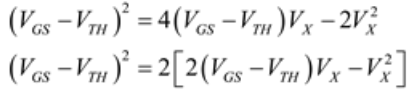
\includegraphics{2.16-14}
	\end{minipage}
\end{figure}

\begin{figure}[H] %H为当前位置,!htb为忽略美学标准,htbp为浮动图形
	\begin{minipage}{\linewidth}
		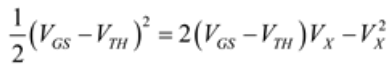
\includegraphics{2.16-15}
	\end{minipage}
\end{figure}

将上式代入\ding{173}

\begin{figure}[H] %H为当前位置,!htb为忽略美学标准,htbp为浮动图形
	\begin{minipage}{\linewidth}
		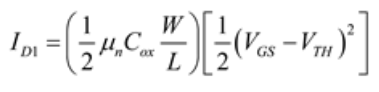
\includegraphics{2.16-16}
	\end{minipage}
\end{figure}

\begin{figure}[H] %H为当前位置,!htb为忽略美学标准,htbp为浮动图形
	\begin{minipage}{\linewidth}
		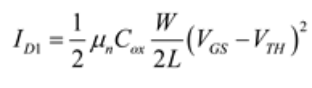
\includegraphics{2.16-17}
	\end{minipage}
\end{figure}

因为$I_{D1}=I_{D2}$,所以

\begin{figure}[H] %H为当前位置,!htb为忽略美学标准,htbp为浮动图形
	\begin{minipage}{\linewidth}
		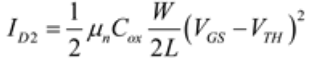
\includegraphics{2.16-18}
	\end{minipage}
\end{figure}

考虑原始饱和区漏电流公式

\begin{figure}[H] %H为当前位置,!htb为忽略美学标准,htbp为浮动图形
	\begin{minipage}{\linewidth}
		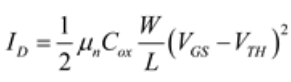
\includegraphics{2.16-19}
	\end{minipage}
\end{figure}

对比以上三式可得把整个图1电路视作一个晶体管时宽长比为$\frac{W}{2L}$。

\scalebox{3}{(3)}

为了保证$M_2$开,要$V_{GS2}>V_{TH}$即$V_{GS}-V_X>V_{TH}$,所以$V_{GS}-V_{TH}>V_X$,即$M_1$一定在线性区

\color{green}{
	
%	\{
%	
%	由图1得此时$M_2$在线性区
%	
%	如果$M_2$在饱和区时$M_1$一定在饱和区
%	
%	
%	\}
	
}

\color{black}{}